%%%%%%%%%%%%%%%%%%%%%%%%%%%%%%%%%%%%%%%%%
% Jacobs Landscape Poster
% LaTeX Template
% Version 1.1 (14/06/14)
%
% Created by:
% Computational Physics and Biophysics Group, Jacobs University
% https://teamwork.jacobs-university.de:8443/confluence/display/CoPandBiG/LaTeX+Poster
% 
% Further modified by:
% Nathaniel Johnston (nathaniel@njohnston.ca)
%
% This template has been downloaded from:
% http://www.LaTeXTemplates.com
%
% License:
% CC BY-NC-SA 3.0 (http://creativecommons.org/licenses/by-nc-sa/3.0/)
%
%%%%%%%%%%%%%%%%%%%%%%%%%%%%%%%%%%%%%%%%%

%----------------------------------------------------------------------------------------
%	PACKAGES AND OTHER DOCUMENT CONFIGURATIONS
%----------------------------------------------------------------------------------------

\documentclass[final]{beamer}

\usepackage[scale=1.0]{beamerposter} % Use the beamerposter package for laying out the poster
\usepackage[acronym,toc]{glossaries}
\newacronym[longplural={metric tons of heavy metal}]{MTHM}{MTHM}{metric ton of heavy metal}
\newacronym{ABM}{ABM}{agent-based modeling}
\newacronym{ACDIS}{ACDIS}{Program in Arms Control \& Domestic and International Security}
\newacronym{AHTR}{AHTR}{Advanced High Temperature Reactor}
\newacronym{ANDRA}{ANDRA}{Agence Nationale pour la gestion des D\'echets RAdioactifs, the French National Agency for Radioactive Waste Management}
\newacronym{ANL}{ANL}{Argonne National Laboratory}
\newacronym{API}{API}{application programming interface}
\newacronym{ARCH}{ARCH}{autoregressive conditional heteroskedastic}
\newacronym{ARE}{ARE}{Aircraft Reactor Experiment}
\newacronym{ARFC}{ARFC}{Advanced Reactors and Fuel Cycles}
\newacronym{ARMA}{ARMA}{autoregressive moving average}
\newacronym{ASME}{ASME}{American Society of Mechanical Engineers}
\newacronym{ATWS}{ATWS}{Anticipated Transient Without Scram}
\newacronym{BDBE}{BDBE}{Beyond Design Basis Event}
\newacronym{BIDS}{BIDS}{Berkeley Institute for Data Science}
\newacronym{BOL}{BOL}{Beginning-of-Life}
\newacronym{BSD}{BSD}{Berkeley Software Distribution}
\newacronym{CAFCA}{CAFCA}{ Code for Advanced Fuel Cycles Assessment }
\newacronym{CASL}{CASL}{Consortium for Advanced Simulation of Light Water Reactors}
\newacronym{CDTN}{CDTN}{Centro de Desenvolvimento da Tecnologia Nuclear}
\newacronym{CEA}{CEA}{Commissariat \`a l'\'Energie Atomique et aux \'Energies Alternatives}
\newacronym{CI}{CI}{continuous integration}
\newacronym{CNEC}{CNEC}{Consortium for Nonproliferation Enabling Capabilities}
\newacronym{CNEN}{CNEN}{Comiss\~{a}o Nacional de Energia Nuclear}
\newacronym{CNERG}{CNERG}{Computational Nuclear Engineering Research Group}
\newacronym{COSI}{COSI}{Commelini-Sicard}
\newacronym{COTS}{COTS}{commercial, off-the-shelf}
\newacronym{CSNF}{CSNF}{commercial spent nuclear fuel}
\newacronym{CTAH}{CTAHs}{Coiled Tube Air Heaters}
\newacronym{CUBIT}{CUBIT}{CUBIT Geometry and Mesh Generation Toolkit}
\newacronym{CURIE}{CURIE}{Centralized Used Fuel Resource for Information Exchange}
\newacronym{DAG}{DAG}{directed acyclic graph}
\newacronym{DANESS}{DANESS}{Dynamic Analysis of Nuclear Energy System Strategies}
\newacronym{DBE}{DBE}{Design Basis Event}
\newacronym{DESAE}{DESAE}{Dynamic Analysis of Nuclear Energy Systems Strategies}
\newacronym{DHS}{DHS}{Department of Homeland Security}
\newacronym{DOE}{DOE}{Department of Energy}
\newacronym{DRACS}{DRACS}{Direct Reactor Auxiliary Cooling System}
\newacronym{DRE}{DRE}{dynamic resource exchange}
\newacronym{DSNF}{DSNF}{DOE spent nuclear fuel}
\newacronym{DYMOND}{DYMOND}{Dynamic Model of Nuclear Development }
\newacronym{EBS}{EBS}{Engineered Barrier System}
\newacronym{EDZ}{EDZ}{Excavation Disturbed Zone}
\newacronym{EIA}{EIA}{U.S. Energy Information Administration}
\newacronym{EPA}{EPA}{Environmental Protection Agency}
\newacronym{EP}{EP}{Engineering Physics}
\newacronym{FCO}{FCO}{Fuel Cycle Options}
\newacronym{FCT}{FCT}{Fuel Cycle Technology}
\newacronym{FCWMD}{FCWMD}{Fuel Cycle and Waste Management Division}
\newacronym{FEHM}{FEHM}{Finite Element Heat and Mass Transfer}
\newacronym{FEPs}{FEPs}{Features, Events, and Processes}
\newacronym{FHR}{FHR}{Fluoride-Salt-Cooled High-Temperature Reactor}
\newacronym{FLiBe}{FLiBe}{Fluoride-Lithium-Beryllium}
\newacronym{GCAM}{GCAM}{Global Change Assessment Model}
\newacronym{GDSE}{GDSE}{Generic Disposal System Environment}
\newacronym{GDSM}{GDSM}{Generic Disposal System Model}
\newacronym{GENIUSv1}{GENIUSv1}{Global Evaluation of Nuclear Infrastructure Utilization Scenarios, Version 1}
\newacronym{GENIUSv2}{GENIUSv2}{Global Evaluation of Nuclear Infrastructure Utilization Scenarios, Version 2}
\newacronym{GENIUS}{GENIUS}{Global Evaluation of Nuclear Infrastructure Utilization Scenarios}
\newacronym{GPAM}{GPAM}{Generic Performance Assessment Model}
\newacronym{GRSAC}{GRSAC}{Graphite Reactor Severe Accident Code}
\newacronym{GUI}{GUI}{graphical user interface}
\newacronym{HLW}{HLW}{high level waste}
\newacronym{HPC}{HPC}{high-performance computing}
\newacronym{HTC}{HTC}{high-throughput computing}
\newacronym{HTGR}{HTGR}{High Temperature Gas-Cooled Reactor}
\newacronym{IAEA}{IAEA}{International Atomic Energy Agency}
\newacronym{IEMA}{IEMA}{Illinois Emergency Mangament Agency}
\newacronym{INL}{INL}{Idaho National Laboratory}
\newacronym{IPRR1}{IRP-R1}{Instituto de Pesquisas Radioativas Reator 1}
\newacronym{IRP}{IRP}{Integrated Research Project}
\newacronym{ISFSI}{ISFSI}{Independent Spent Fuel Storage Installation}
\newacronym{ISRG}{ISRG}{Independent Student Research Group}
\newacronym{JFNK}{JFNK}{Jacobian-Free Newton Krylov}
\newacronym{LANL}{LANL}{Los Alamos National Laboratory}
\newacronym{LBNL}{LBNL}{Lawrence Berkeley National Laboratory}
\newacronym{LCOE}{LCOE}{levelized cost of electricity}
\newacronym{LDRD}{LDRD}{laboratory directed research and development}
\newacronym{LFR}{LFR}{Lead-Cooled Fast Reactor}
\newacronym{LGPL}{LGPL}{Lesser GNU Public License}
\newacronym{LLNL}{LLNL}{Lawrence Livermore National Laboratory}
\newacronym{LMFBR}{LMFBR}{Liquid-Metal-cooled Fast Breeder Reactor}
\newacronym{LOFC}{LOFC}{Loss of Forced Cooling}
\newacronym{LOHS}{LOHS}{Loss of Heat Sink}
\newacronym{LOLA}{LOLA}{Loss of Large Area}
\newacronym{LP}{LP}{linear program}
\newacronym{LWR}{LWR}{Light Water Reactor}
\newacronym{MARKAL}{MARKAL}{MARKet and ALlocation}
\newacronym{MA}{MA}{minor actinide}
\newacronym{MCNP}{MCNP}{Monte Carlo N-Particle code}
\newacronym{MILP}{MILP}{mixed-integer linear program}
\newacronym{MIT}{MIT}{the Massachusetts Institute of Technology}
\newacronym{MOAB}{MOAB}{Mesh-Oriented datABase}
\newacronym{MOOSE}{MOOSE}{Multiphysics Object-Oriented Simulation Environment}
\newacronym{MOX}{MOX}{mixed oxide}
\newacronym{MSBR}{MSBR}{Molten Salt Breeder Reactor}
\newacronym{MSRE}{MSRE}{Molten Salt Reactor Experiment}
\newacronym{MSR}{MSR}{Molten Salt Reactor}
\newacronym{NAGRA}{NAGRA}{National Cooperative for the Disposal of Radioactive Waste}
\newacronym{NCSA}{NCSA}{National Center for Supercomputing Applications}
\newacronym{NEAMS}{NEAMS}{Nuclear Engineering Advanced Modeling and Simulation}
\newacronym{NEUP}{NEUP}{Nuclear Energy University Programs}
\newacronym{NFCSim}{NFCSim}{Nuclear Fuel Cycle Simulator}
\newacronym{NFC}{NFC}{Nuclear Fuel Cycle}
\newacronym{NGNP}{NGNP}{Next Generation Nuclear Plant}
\newacronym{NMWPC}{NMWPC}{Nuclear MW Per Capita}
\newacronym{NNSA}{NNSA}{National Nuclear Security Administration}
\newacronym{NPRE}{NPRE}{Department of Nuclear, Plasma, and Radiological Engineering}
\newacronym{NQA1}{NQA-1}{Nuclear Quality Assurance - 1}
\newacronym{NRC}{NRC}{Nuclear Regulatory Commission}
\newacronym{NSF}{NSF}{National Science Foundation}
\newacronym{NSSC}{NSSC}{Nuclear Science and Security Consortium}
\newacronym{NUWASTE}{NUWASTE}{Nuclear Waste Assessment System for Technical Evaluation}
\newacronym{NWF}{NWF}{Nuclear Waste Fund}
\newacronym{NWTRB}{NWTRB}{Nuclear Waste Technical Review Board}
\newacronym{OCRWM}{OCRWM}{Office of Civilian Radioactive Waste Management}
\newacronym{ORION}{ORION}{ORION}
\newacronym{ORNL}{ORNL}{Oak Ridge National Laboratory}
\newacronym{PARCS}{PARCS}{Purdue Advanced Reactor Core Simulator}
\newacronym{PBAHTR}{PB-AHTR}{Pebble Bed Advanced High Temperature Reactor}
\newacronym{PBFHR}{PB-FHR}{Pebble-Bed Fluoride-Salt-Cooled High-Temperature Reactor}
\newacronym{PEI}{PEI}{Peak Environmental Impact}
\newacronym{PH}{PRONGHORN}{PRONGHORN}
\newacronym{PI}{PI}{Principal Investigator}
\newacronym{PNNL}{PNNL}{Pacific Northwest National Laboratory}
\newacronym{PRIS}{PRIS}{Power Reactor Information System}
\newacronym{PRKE}{PRKE}{Point Reactor Kinetics Equations}
\newacronym{PSPG}{PSPG}{Pressure-Stabilizing/Petrov-Galerkin}
\newacronym{PWAR}{PWAR}{Pratt and Whitney Aircraft Reactor}
\newacronym{PWR}{PWR}{Pressurized Water Reactor}
\newacronym{PyNE}{PyNE}{Python toolkit for Nuclear Engineering}
\newacronym{PyRK}{PyRK}{Python for Reactor Kinetics}
\newacronym{QA}{QA}{quality assurance}
\newacronym{RDD}{RD\&D}{Research Development and Demonstration}
\newacronym{RD}{R\&D}{Research and Development}
\newacronym{RELAP}{RELAP}{Reactor Excursion and Leak Analysis Program}
\newacronym{RIA}{RIA}{Reactivity Insertion Accident}
\newacronym{RIF}{RIF}{Region-Institution-Facility}
\newacronym{SAM}{SAM}{Simulation and Modeling}
\newacronym{SCF}{SCF}{Software Carpentry Foundation}
\newacronym{SFR}{SFR}{Sodium-Cooled Fast Reactor}
\newacronym{SINDAG}{SINDA{\textbackslash}G}{Systems Improved Numerical Differencing Analyzer $\backslash$ Gaski}
\newacronym{SKB}{SKB}{Svensk K\"{a}rnbr\"{a}nslehantering AB}
\newacronym{SNF}{SNF}{spent nuclear fuel}
\newacronym{SNL}{SNL}{Sandia National Laboratory}
\newacronym{SNM}{SNM}{Special Nuclear Material}
\newacronym{STC}{STC}{specific temperature change}
\newacronym{SUPG}{SUPG}{Streamline-Upwind/Petrov-Galerkin}
\newacronym{SWF}{SWF}{Separations and Waste Forms}
\newacronym{SWU}{SWU}{Separative Work Unit}
\newacronym{SandO}{S\&O}{Signatures and Observables}
\newacronym{THW}{THW}{The Hacker Within}
\newacronym{TRIGA}{TRIGA}{Training Research Isotope General Atomic}
\newacronym{TRISO}{TRISO}{Tristructural Isotropic}
\newacronym{TSM}{TSM}{Total System Model}
\newacronym{TSPA}{TSPA}{Total System Performance Assessment for the Yucca Mountain License Application}
\newacronym{UDB}{UDB}{Unified Database}
\newacronym{UFD}{UFD}{Used Fuel Disposition}
\newacronym{UML}{UML}{Unified Modeling Language}
\newacronym{UNFSTANDARDS}{UNFST\&DARDS}{Used Nuclear Fuel Storage, Transportation \& Disposal Analysis Resource and Data System}
\newacronym{UOX}{UOX}{uranium oxide}
\newacronym{UQ}{UQ}{uncertainty quantification}
\newacronym{US}{US}{United States}
\newacronym{UW}{UW}{University of Wisconsin}
\newacronym{VISION}{VISION}{the Verifiable Fuel Cycle Simulation Model}
\newacronym{VV}{V\&V}{verification and validation}
\newacronym{WIPP}{WIPP}{Waste Isolation Pilot Plant}
\newacronym{YMG}{YMG}{Young Members Group}
\newacronym{YMR}{YMR}{Yucca Mountain Repository Site}
\newacronym{NEI}{NEI}{Nuclear Energy Institute}
%\newacronym{<++>}{<++>}{<++>}
%\newacronym{<++>}{<++>}{<++>}

\usetheme{confposter} % Use the confposter theme supplied with this template

\setbeamercolor{block title}{fg=dblue!80,bg=white} % Colors of the block titles
\setbeamercolor{block body}{fg=black,bg=white} % Colors of the body of blocks
\setbeamercolor{block alerted title}{fg=white,bg=dblue!70} % Colors of the highlighted block titles
\setbeamercolor{block alerted body}{fg=black,bg=dblue!10} % Colors of the body of highlighted blocks
% Many more colors are available for use in beamerthemeconfposter.sty

%-----------------------------------------------------------
% Define the column widths and overall poster size
% To set effective sepwid, onecolwid and twocolwid values, first choose how many columns you want and how much separation you want between columns
% In this template, the separation width chosen is 0.024 of the paper width and a 4-column layout
% onecolwid should therefore be (1-(# of columns+1)*sepwid)/# of columns e.g. (1-(4+1)*0.024)/4 = 0.22
% onecolwid should therefore be (1-(# of columns+1)*sepwid)/# of columns e.g. 
% (1-(3+1)*0.025)/3 = 0.3
% Set twocolwid to be (2*onecolwid)+sepwid = 0.464
% Set threecolwid to be (3*onecolwid)+2*sepwid = 0.708

\newlength{\sepwid}
\newlength{\onecolwid}
\newlength{\twocolwid}
\newlength{\threecolwid}
\setlength{\paperwidth}{36in} % A0 width: 46.8in
\setlength{\paperheight}{48in} % A0 height: 33.1in
\setlength{\textwidth}{34in} % A0 width: 46.8in
\setlength{\textheight}{46in} % A0 height: 33.1in
\setlength{\sepwid}{0.025\paperwidth} % Separation width (white space) between columns
\setlength{\onecolwid}{0.3\paperwidth} % Width of one column
\setlength{\twocolwid}{0.625\paperwidth} % Width of two columns
\setlength{\threecolwid}{0.95\paperwidth} % Width of three columns
\setlength{\topmargin}{-0.5in} % Reduce the top margin size
%-----------------------------------------------------------

\usepackage{graphicx}  % Required for including images
\newcommand{\Cyclus}{\textsc{Cyclus}\xspace}%

\usepackage{tabularx}
\newcolumntype{b}{X}
\newcolumntype{s}{>{\hsize=.5\hsize}X}
\newcolumntype{m}{>{\hsize=.75\hsize}X}
\newcolumntype{z}{>{\hsize=.65\hsize}X}

\usepackage{booktabs} % Top and bottom rules for tables
\usepackage{xspace}
\usepackage{amsmath}
\usepackage{bigints}

\setbeamertemplate{bibliography item}[text]

%----------------------------------------------------------------------------------------
%	TITLE SECTION 
%----------------------------------------------------------------------------------------

\title{
	
\includegraphics[width=0.3\linewidth]{UIUC_Logo}
	\vspace{2cm}
	\hspace{50cm}
	\vspace{1cm}
	Simulation of Spent Nuclear Fuel loading into a Final Waste Repository
} % Poster title

\author{\textbf{Gwendolyn J. Chee}, Kathryn D. Huff}
\institute{University of Illinios at Urbana-Champaign, Department of Nuclear, Plasma, and Radiological Engineering, Urbana, IL 61801}
%----------------------------------------------------------------------------------------

\begin{document}

\addtobeamertemplate{block end}{}{\vspace*{2ex}} % White space under blocks
\addtobeamertemplate{block alerted end}{}{\vspace*{2ex}} % White space under highlighted (alert) blocks

\setlength{\belowcaptionskip}{2ex} % White space under figures
\setlength\belowdisplayshortskip{2ex} % White space under equations

\begin{frame}[t] % The whole poster is enclosed in one beamer frame

\begin{columns}[t,totalwidth=\threecolwid] % The whole poster consists of three major columns, the second of which is split into two columns twice - the [t] option aligns each column's content to the top

\begin{column}{0.5\sepwid}\end{column} % Empty spacer column

\begin{column}{\onecolwid} % The first column

%----------------------------------------------------------------------------------------
%	OBJECTIVES
%----------------------------------------------------------------------------------------
\setbeamercolor{block alerted title}{fg=black,bg=norange} % Change the alert block title colors
\setbeamercolor{block alerted body}{fg=black,bg=white} % Change the alert block body colors
\begin{alertblock}{Objectives}
\begin{itemize}
        \item Create a \Cyclus Waste Conditioning Model that packages spent fuel 
        bundles into canisters which have user-defined properties. 
		\item Create a \Cyclus Medium-Fidelity Repository Model that gives accurate 
		time and spatial dependent temperature values and loads the repository
		based on a user-selected loading strategy. 
\end{itemize}

\end{alertblock}

%----------------------------------------------------------------------------------------
%	MOTIVATION
%----------------------------------------------------------------------------------------

\begin{block}{Motivation}
Previous work in studying repository loading have used spent fuel assemblies 
that have an average burn up composition \cite{johnson_optimizing_2016} 
to evaluate the heat load in the repository \cite{greenberg_application_2012}.
Instead of using average \gls{SNF} composition, this work aims to use \textbf{U.S. 
historical SNF inventory data} \cite{peterson_unf_standards_2017} in various 
simulations to study how waste acceptance strategies impact repository loading.
The \gls{UDB} contains assembly-specific data including initial enrichment, 
burnup, \gls{MTHM}, assembly type and discharge date \cite{peterson_fuel_2015}. 
Irradiation and decay calculations using SCALE \cite{bowman_scale_2011} were 
performed on each spent fuel assembly based on the previously mentioned 
parameters in the collected data to obtain mass, heat, activity and isotopic 
composition for each assembly \cite{peterson_additional_2017}. 
This data is input into \Cyclus using the UDB reactor agent \cite{}. 
\Cyclus is capable of tracking discrete isotopes and their time-dependent decay. 
With these capabilities, we can more accurately study the dynamic loading 
of a waste repository. 

\end{block}

%----------------------------------------------------------------------------------------
%	Cyclus
%----------------------------------------------------------------------------------------

\begin{block}{Cyclus}
\Cyclus is an agent-based extensible framework for modeling flow of material 
through user-defined nuclear fuel cycles \cite{huff_fundamental_2016}. 
In \Cyclus, each facility in the fuel cycle is modeled individually 
and they interact with one another as independent \textit{agents}. 
The goal of this work is to develop a waste conditioning \textit{facility agent} 
and a waste repository \textit{facility agent} to provide \Cyclus with 
the capabilities to run simulations to study how waste acceptance 
strategies impact repository loading. 
\begin{figure}
	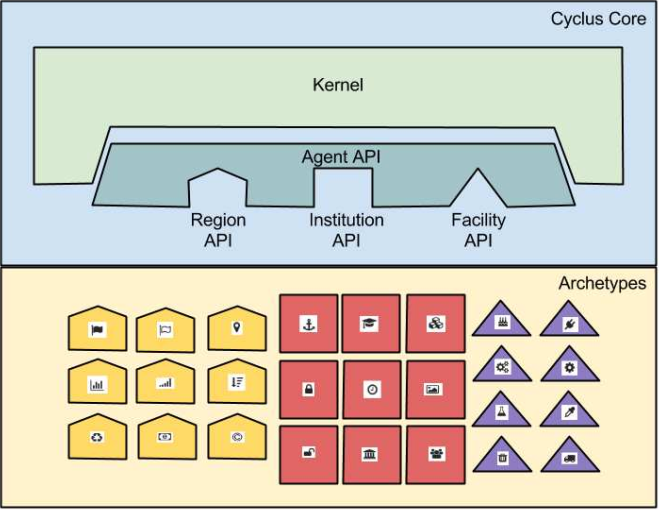
\includegraphics[width=0.9\linewidth]{Cyclus_graph}
	\caption{\Cyclus API allows for modular build of simulations \cite{huff_fundamental_2016}}
\end{figure}

\end{block}

\begin{block}{Waste Conditioning Model}
	The waste conditioning model accepts spent fuel bundles and puts them into a cylindrical
	waste canister. The model allows the user to define one or two canister material layers. 
	
	In the waste conditioning model, the user can define the variables:  
		\begin{itemize}
			\item Number of spent fuel bundles in each canister 
			\item Thermal Conductivity of canister material layers 
			\item Thermal Diffusivity of Canister 
			\item Radius and height of Canister
		\end{itemize}
	
	\end{block}

%----------------------------------------------------------------------------------------

\end{column} % End of the first column

\begin{column}{\sepwid}\end{column} % Empty spacer column


%----------------------------------------------------------------------------------------

\begin{column}{\onecolwid} % The second column
%----------------------------------------------------------------------------------------
%	MODELS
%----------------------------------------------------------------------------------------

\begin{block}{Waste Repository Model}
The waste repository model accepts waste canisters and emplaces the canisters into 
available positions within the waste repository based on a thermal criteria. 
If the thermal criteria is not met, the waste canister will be placed into a buffer 
until it meets the thermal criteria.  
The thermal criteria is set by the repository host geology. 
It is the temperature limit applied at the interface between waste package surface 
and the host geology. 

Table \ref{tab:temp_limit} shows the temperature limits, thermal conductivity 
and thermal diffusivity for the host geology included in this study. 

\begin{table}[]
	\label{tab:temp_limit}
	\caption{Temperature limit at interface between waste package surface 
	and each host geology \cite{sutton_investigations_2011}}
	\begin{tabular}{|l|l|l|l|}
	\hline
	Rock Type & $T_{limit}$ [$^\circ$C] & k [$\frac{W}{mK}$] &  $\alpha$ [$\frac{m^2}{s}$]  \\ \hline
	Granite   & 100 & 2.5  & 1.13\\ \hline
	Clay      & 100 & 1.75 & 6.45\\ \hline
	Salt      & 200 & 4.2  & 2.07\\ \hline
	\end{tabular}
\end{table}

In the waste repository model, the user can define the variables: 
	\begin{itemize}
		\item Distance between waste canisters
		\item Distance between drifts 
		\item Repository host geology 
		\item Loading Strategy 
	\end{itemize}

\textbf{Thermal Model}

At each time step, the waste repository model recalculates the temperature at each 
location in the repository after the addition of new waste packages. 
To accurately determine the temperature in the repository, a the thermal model that 
relies on a transient 'outside' model and quasi-steady-state 'inside' model is used. 
[Reason for inside and outside model]

\textbf{Transient Outside Model}

Figure \ref{fig:conceptual_layout} shows the conceptual layout of the central waste package 
and the adjacent point and line sources. 

\begin{figure}
	\label{fig:conceptual_layout}
	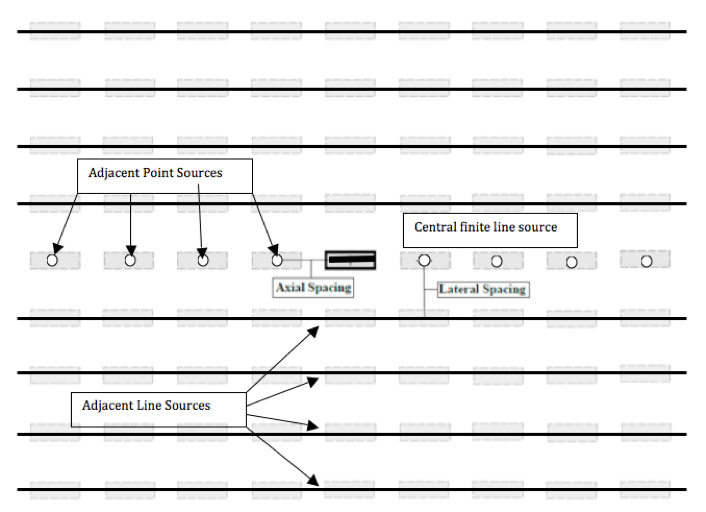
\includegraphics[width=0.9\linewidth]{outsidemodel}
	\caption{Conceptual layout}
\end{figure}

Temperature solutions for the central waste package, adjacent point and line sources 
are superimposed to calculate the temperature at specific points in the repository.
The equations for calculating temperature of each contributing component 
are included below. 

The central drift consists of one finite line source which represents the central 
waste package. 
\begin{align*}
	T_{line}(t,x,y,z) &= \frac{1}{8 \pi k}  \int_{0}^{t} \frac{q_L(t')}{t-t'}e^{\frac{-(x^2+z^2)}{4\alpha(t-t')}} \\
	&[erf[\frac{1}{2}\frac{y+L/2}{\sqrt{\alpha(t-t')}}]-erf[\frac{1}{2}\frac{y-L/2}{\sqrt{\alpha(t-t')}}]] dt'
\end{align*}
The central drift also consists of point sources that represent neighboring 
waste packages in the central drift. 
\begin{align*}
	T_{point}(t,r) = \frac{1}{8 k \sqrt{\alpha} \pi^{3/2}} \int_{0}^{t}\frac{q(t')}{(t-t')^{3/2}}e^{\frac{-r^2}{4\alpha(t-t')}}dt'
\end{align*}
The neighboring drifts are represented by infinite line sources.  
\begin{align*}
	T_{\infty line}(t,x,z) = \frac{1}{4\pi k} \int_0^t \frac{q_L(t')}{t-t'} e^{\frac{-(x^2+z^2)}{4\alpha (t-t')}} dt'
\end{align*}

\textbf{Quasi-steady-state 'inside' model}

\end{block}


%----------------------------------------------------------------------------------------

\end{column} % End of column 2

\begin{column}{\sepwid}\end{column} % Empty spacer column

\begin{column}{\onecolwid} % The third column
	
%----------------------------------------------------------------------------------------
%	FUTURE WORK
%----------------------------------------------------------------------------------------

\begin{alertblock}{Future Work}


\end{alertblock}





%----------------------------------------------------------------------------------------
%	ACKNOWLEDGEMENTS
%----------------------------------------------------------------------------------------

\setbeamercolor{block title}{fg=norange,bg=white} % Change the block title color

\begin{block}{Acknowledgements}
	
	This research is being performed using funding received from the DOE Office
	of Nuclear Energy's NEUP
	(Project 16-10512) 'Demand-Driven Cycamore Archetypes'.
	
	
\end{block}

%----------------------------------------------------------------------------------------
%	CONTACT INFORMATION
%----------------------------------------------------------------------------------------

\setbeamercolor{block alerted title}{fg=black,bg=norange} % Change the alert block title colors
\setbeamercolor{block alerted body}{fg=black,bg=white} % Change the alert block body colors



\begin{block}{References}

	{\footnotesize\bibliographystyle{abbrv} 
	\bibliography{poster}}
\end{block}


%----------------------------------------------------------------------------------------



\end{column} % End of the third column

\end{columns} % End of all the columns in the poster

\end{frame} % End of the enclosing frame

\end{document}
\begin{column}{\sepwid}\end{column} % Empty spacer column
